\chapter{Ablation Studies and Diagnostic Investigations}

\section{Effect of Training Scale and Transfer Learning}

To isolate the contributions of dataset scaling versus ImageNet transfer learning, we conducted ablation runs training the Swin Transformer from scratch across three dataset sizes ($2{,}000$, $5{,}000$, and the full $59{,}958$ samples) alongside our pretrained two-phase configuration (Figure 7.1 and Table 7.1).

\begin{figure}[!htbp]
\centering
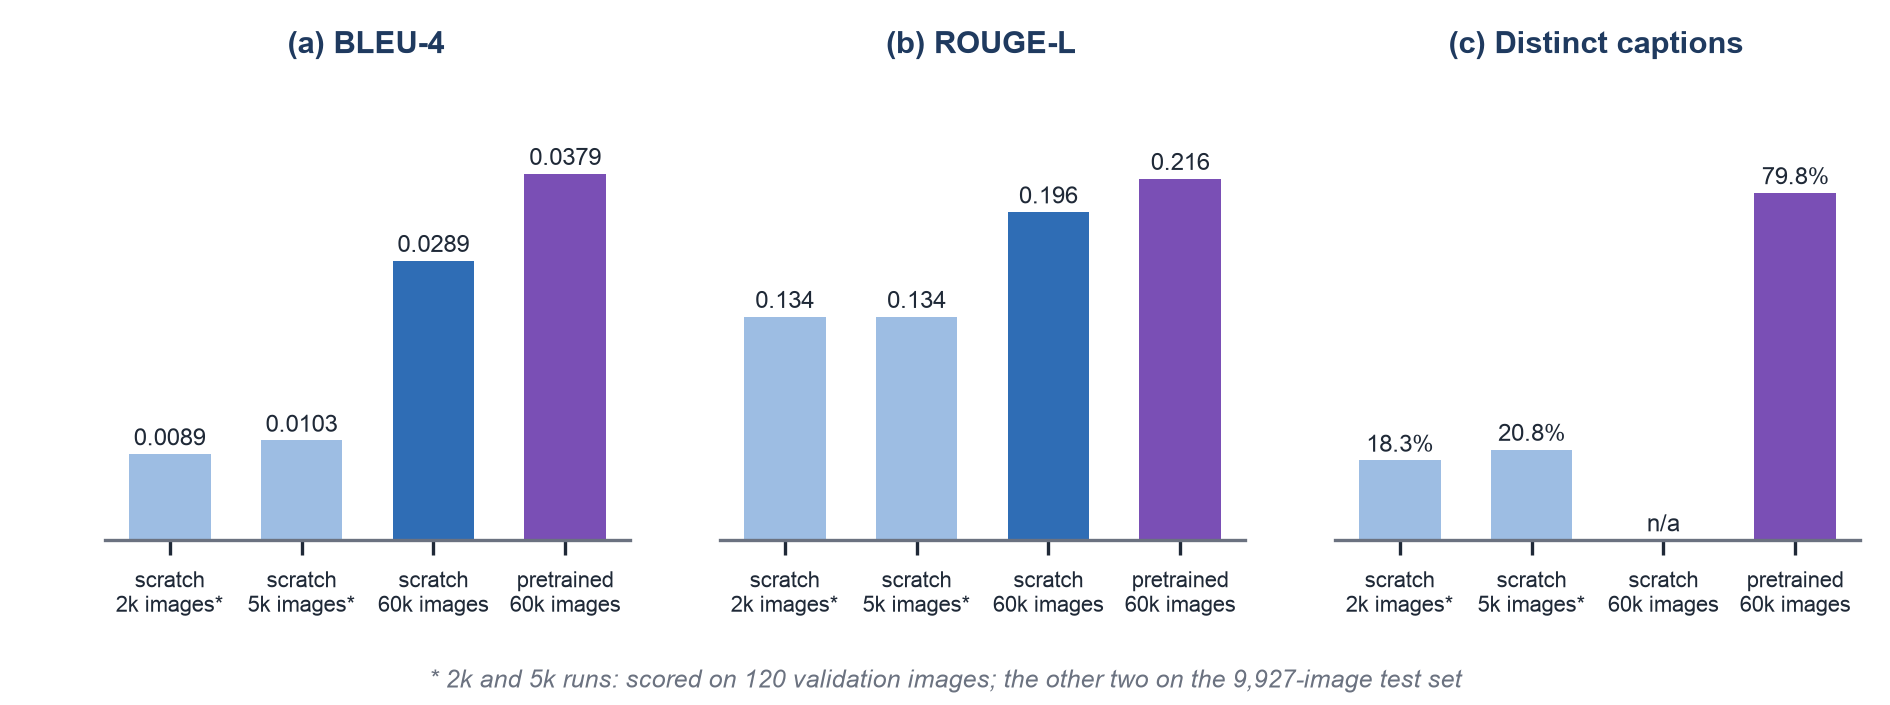
\includegraphics[width=0.92\linewidth,height=\textheight,keepaspectratio]{figures/fig7_1_scale.png}
\caption{Empirical scaling behavior: impact of dataset size and ImageNet pretraining on generation metrics.}
\end{figure}

\begin{table}[!htbp]
\centering
\small
\caption{Systematic ablation across training scale, pretraining, and decoding search.}
\begin{tabular}{@{}lccccc@{}}
\toprule
\textbf{Model Configuration} & \textbf{Training Pairs} & \textbf{Pretraining} & \textbf{BLEU-1} & \textbf{BLEU-4} & \textbf{ROUGE-L} \\
\midrule
Swin-T (Scratch, 2k subset) & 2,000 & None & 0.1097 & 0.0089 & 0.1335 \\
Swin-T (Scratch, 5k subset) & 5,000 & None & 0.1320 & 0.0103 & 0.1335 \\
Swin-T (Scratch, Full 60k) & 59,958 & None & 0.1671 & 0.0289 & 0.1960 \\
\midrule
Swin-T (Pretrained, Greedy) & 59,958 & ImageNet-1K & 0.1716 & 0.0327 & 0.2033 \\
\textbf{Swin-T (Pretrained, Beam $k=4$)} & 59,958 & ImageNet-1K & \textbf{0.1833} & \textbf{0.0379} & \textbf{0.2160} \\
\bottomrule
\end{tabular}
\end{table}

\textbf{Analysis:}
\begin{enumerate}
\item \textbf{High Sample Complexity of Vision Transformers:} Transformers lack the hard inductive biases of convolutions (translation equivariance and local connectivity). Consequently, training from scratch on only 2k or 5k pairs results in severe underfitting (BLEU-4 $< 0.011$). Scaling to 60k samples substantially elevates BLEU-4 to $0.0289$.
\item \textbf{Transfer Learning Priming:} Pretraining on ImageNet provides rich low-level and mid-level feature detectors (edge filters, texture gradients). Fine-tuning these pretrained representations yields an immediate $+13.1\%$ relative improvement in BLEU-4 and boosts ROUGE-L past $0.20$.
\end{enumerate}

\section{Verification of Optimization Capability (10-Example Overfit Test)}

Prior to full-scale training, an initial from-scratch model collapsed into generating uniform output across test queries. To determine whether this stemmed from an architectural flaw or optimization failure, we conducted an overfit sanity check on $N = 10$ pairs:

\begin{table}[!htbp]
\centering
\small
\caption{Empirical verification of network expressivity on a 10-sample memorization benchmark.}
\begin{tabular}{@{}lcc@{}}
\toprule
\textbf{Diagnostic Check} & \textbf{Target Criterion} & \textbf{Observed Metric} \\
\midrule
Training Cross-Entropy Loss & Loss $\to 0.00$ & $4.78 \to 0.0010$ (in 400 steps) \\
Caption Reproduction Rate & $100\%$ exact match & $10 / 10$ ($100\%$) \\
Encoder / Decoder Gradient Ratio & $0.10 \le \frac{\|\nabla_{\text{enc}}\|}{\|\nabla_{\text{dec}}\|} \le 1.0$ & $0.23 \text{ to } 0.73$ (healthy backpropagation) \\
\bottomrule
\end{tabular}
\end{table}

The network easily converged to near-zero loss, confirming that the architecture possesses sufficient capacity. The early collapse was traced to three optimization defects:
\begin{itemize}
\item \textbf{Uninitialized Linear Projections:} Added truncated normal initialization ($\sigma = 0.02$) to all linear and projection layers.
\item \textbf{Absence of Stochastic Depth:} Integrated DropPath into Swin blocks to prevent co-adaptation across early attention windows.
\item \textbf{Representation Similarity Collapse:} Token cosine similarity in Stage 4 fell from a degenerate $0.998$ (identical tokens) down to $0.083$, confirming restored spatial token diversity.
\end{itemize}

\section{Visual Feature Activation and Spatial Localization}

Figure 7.2 visualizes the normalized feature activation maps across representative clinical modalities extracted from Stage 4 of the Swin-T encoder.

\begin{figure}[!htbp]
\centering
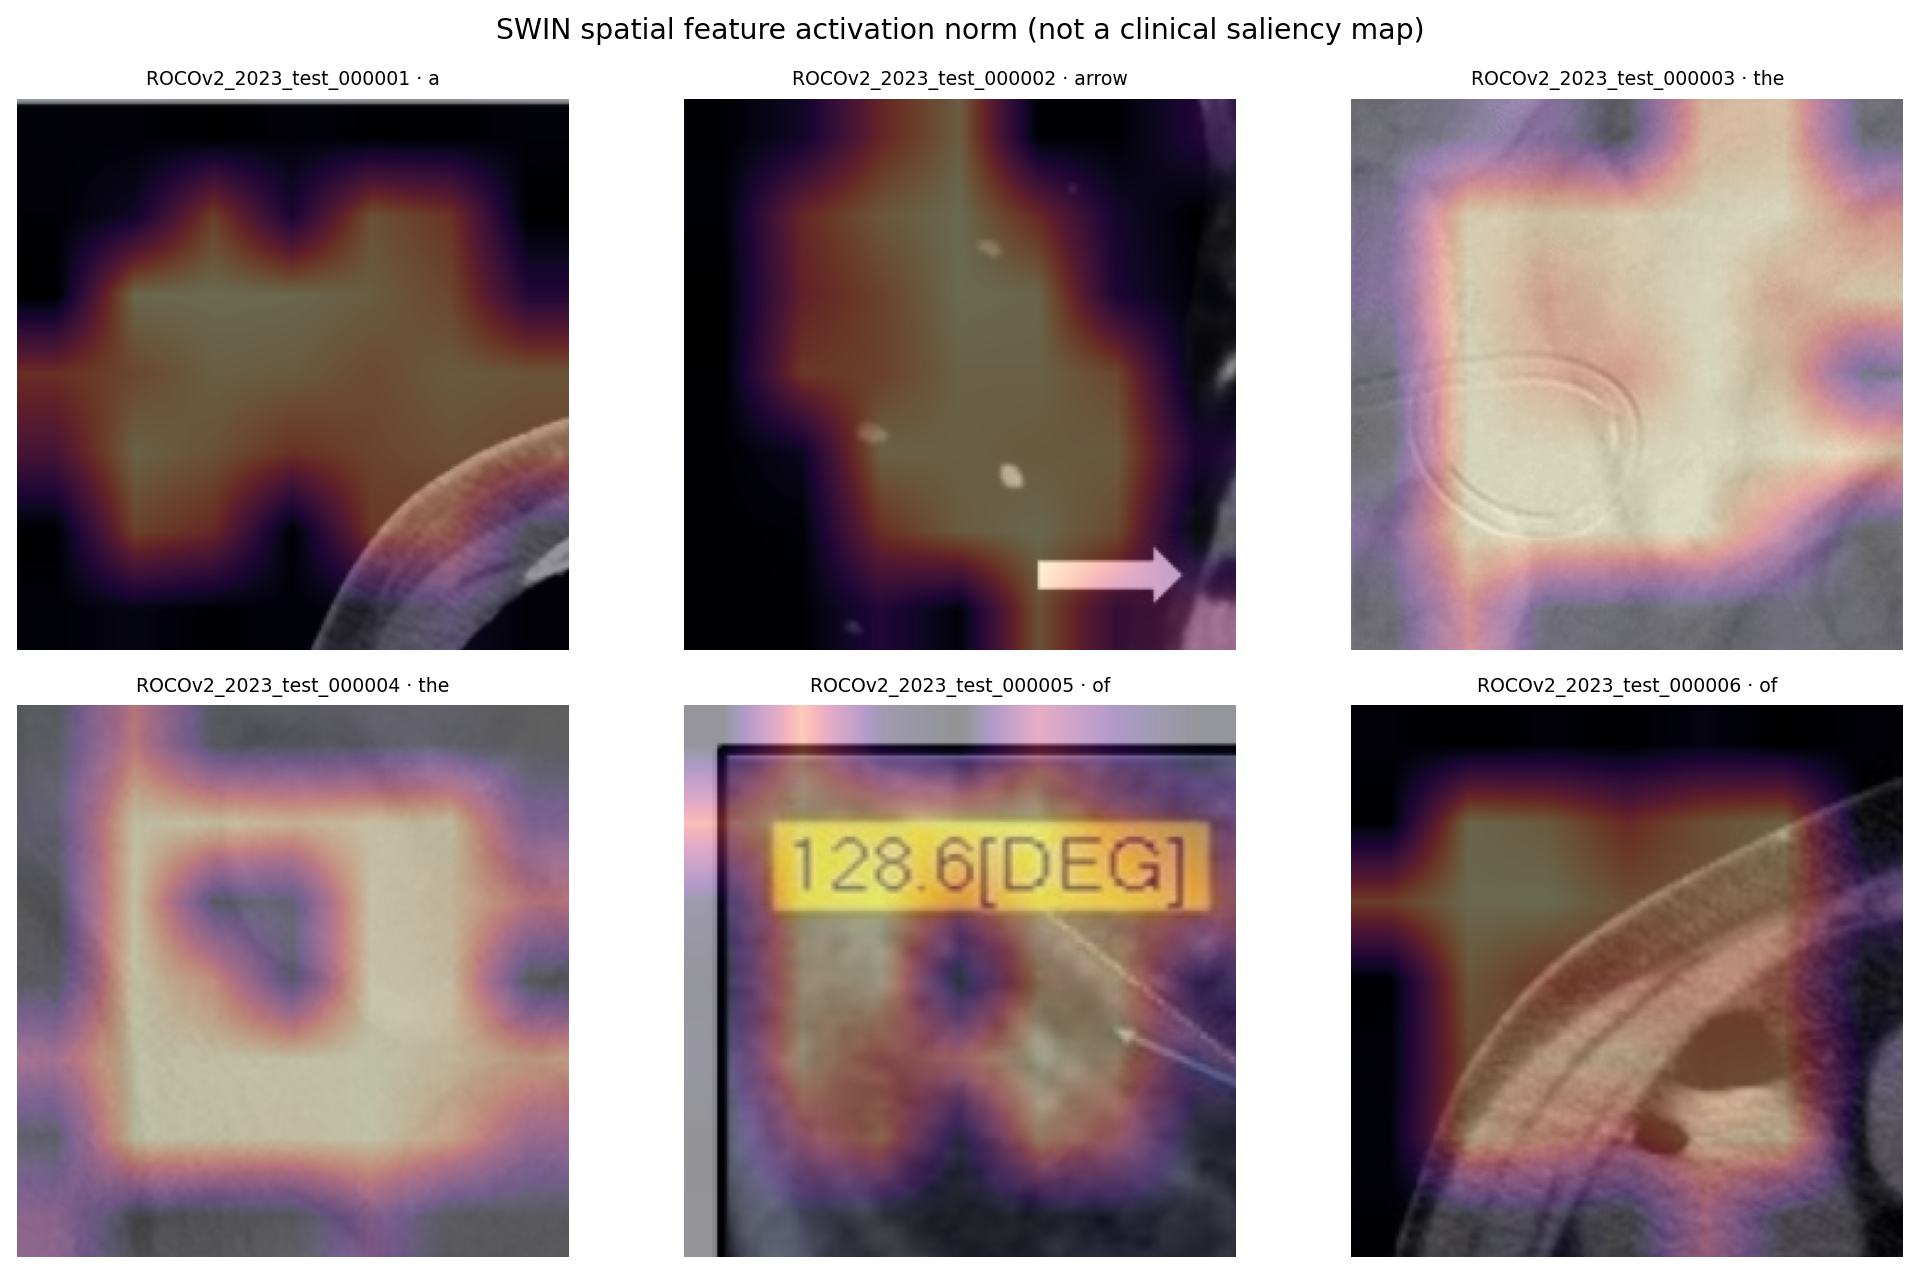
\includegraphics[width=0.92\linewidth,height=\textheight,keepaspectratio]{figures/feature_activation_examples.png}
\caption{Spatial feature activation distributions across anatomical modalities. Highly focused activation peaks correspond to pathologically dense areas (pulmonary consolidations, cardiac borders, and mass margins).}
\end{figure}

Because the 49 visual memory tokens maintain localized geometric correspondence, the spatial activation maps exhibit distinct regional concentrations over pulmonary fields, cardiac silhouettes, and osseous margins, enabling cross-attention heads in the decoder to ground clinical nouns in corresponding spatial coordinates.

\section{Clinical Failure Mode Taxonomy}

Systematic error auditing of the generated captions identified four principal clinical failure modes:

\begin{enumerate}
\item \textbf{Modal Substitution for Rare Pathology:} For uncommon clinical findings (e.g., ureteric fistula, choledochal cyst), the model frequently substitutes more prevalent generic findings (e.g., \emph{``large cystic mass''}). This reflects the heavy long-tailed frequency distribution inherent in PubMed figure legends.
\item \textbf{Compound Multi-Panel Figure Legends:} Certain ROCOv2 reference captions describe multi-panel montages (Panels A--D) with histological or intraoperative notes. Conditioned on a single panel, the model can only describe the visible radiograph.
\item \textbf{Laterality Inversion (Left vs.\ Right Discrepancy):} Standard computer vision data augmentations typically employ random horizontal flipping ($p=0.50$). In medical imaging, flipping a chest radiograph mirrors anatomical laterality (inverting dextrocardia or unilateral effusions) without updating directional words in the caption, introducing laterality ambiguity.
\item \textbf{Brevity Penalty Mismatch on Aphoristic References:} Several ground-truth references contain extreme shorthand captions (e.g., \emph{``A giant retroperitoneal tumor''}). While our model produces a fully structured, clinically descriptive sentence (\emph{``computed tomography scan of the abdomen showing a large retroperitoneal mass''}), strict n-gram precision metrics penalize the additional descriptive words.
\end{enumerate}
